%%%%%%%%%%%%%%%%%%%%%%%%%%%%%%%%%%%%%%%%%%%%%%%%%%%%%%%%%%%%%%
%% LaTeX template for the science justification to be       %%
%%       submitted as part of an ALMA proposal.             %%
%%                                                          %%
%%                      ALMA Cycle 2                        %%
%%                                                          %%
%%%%%%%%%%%%%%%%%%%%%%%%%%%%%%%%%%%%%%%%%%%%%%%%%%%%%%%%%%%%%%

\documentclass[11pt, a4paper, onecolumn]{article}

\usepackage{graphics,graphicx}

% Load commands

\newcommand{\HRule}{\rule{\linewidth}{0.5mm}}
\newcommand{\Hrule}{\rule{\linewidth}{0.3mm}}
\newcommand{\ergseccm}{erg\,s$^{-1}$\,cm$^{-2}$}
\newcommand{\etal}{et\,al.}
\newcommand{\halpha}{H$\alpha$}
\newcommand{\lya}{Ly$\alpha$}
\newcommand{\lsim}{\raise0.3ex\hbox{$<$}\kern-0.75em{\lower0.65ex\hbox{$\sim$}}}
\newcommand{\mjpbeam}{\,\,mJy\,beam$^{-1}$}
\newcommand{\msun}{M$_{\odot}$}

% column densities
\newcommand{\hii}{H\,{\sc ii}}
\newcommand{\hi}{{\rm H\,{\sc i}}}
\newcommand{\nhi}{{$N$(\rm H\,{\sc i})}}
\newcommand{\hiColDens}{{$N($\rm H$_{\rm 2})$}}
\newcommand{\htwo}{{\rm H$_{\rm 2}$}}
\newcommand{\htwoColDens}{{$N($\rm H$_{\rm 2})$}}
\newcommand{\hisd}{$\Sigma_{\rm H\,{\text{\sc i}}}$}
\newcommand{\htwosd}{$\Sigma_{\rm H2}$}
\newcommand{\hsd}{$\Sigma_{\rm H}$}


\newcommand{\ii}{{\sc ii}}
\newcommand{\iii}{{\sc iii}}

% Units
\newcommand{\kms}{km\,s$^{-1}$}
\newcommand{\pom}{\,$\pm$\,}
\newcommand{\mm}{$\mu$m}
\newcommand{\lcdm}{$\Lambda$CDM}
\newcommand{\cm}{cm$^{-2}$}
\newcommand{\colDens}{$\times\ 10^{20}$ cm$^{-2}$}

% Units
\newcommand{\vrot}{$v_{\rm rot}$}
\newcommand{\vdisp}{$\sigma_{\rm HI}$}
\newcommand{\tspin}{$T_{\rm s}$}
\newcommand{\tdust}{$T_{\rm d}$}



% load packages
% Packages

% \usepackage{fancyhdr} % Required for custom headers
% \usepackage{lastpage} % Required to determine the last page for the footer
% \usepackage{extramarks} % Required for headers and footers
% \usepackage[usenames,dvipsnames]{color} % Required for custom colors
\usepackage{graphicx} % Required to insert images
% \usepackage{listings} % Required for insertion of code
% \usepackage{courier} % Required for the courier font
% \usepackage{dsfont} % For special math characters
% \usepackage{verbatim}

%\usepackage{amsmath, amssymb, bm} % For matrix notation
\usepackage[english]{babel}
\usepackage[paperwidth=8.5in,paperheight=11in,margin=1.0in]{geometry}
\usepackage{listings}
\usepackage{hyperref}
%\usepackage[cmex10]{amsmath, bm}
\usepackage{amsmath, bm}
\usepackage{blkarray}








% load formatting
\pdfcompresslevel0

% ==============================================================================
% PYTHON
% ==============================================================================
\usepackage[utf8]{inputenc}

% Default fixed font does not support bold face
\DeclareFixedFont{\ttb}{T1}{txtt}{bx}{n}{12} % for bold
\DeclareFixedFont{\ttm}{T1}{txtt}{m}{n}{12}  % for normal

% Custom colors
\usepackage{color}
\definecolor{deepblue}{rgb}{0,0,0.5}
\definecolor{deepred}{rgb}{0.6,0,0}
\definecolor{deepgreen}{rgb}{0,0.5,0}

\usepackage{listings}

% Python style for highlighting
\newcommand\pythonstyle{\lstset{
language=Python,
basicstyle=\ttm,
otherkeywords={self},             % Add keywords here
keywordstyle=\ttb\color{deepblue},
emph={MyClass,__init__},          % Custom highlighting
emphstyle=\ttb\color{deepred},    % Custom highlighting style
stringstyle=\color{deepgreen},
frame=tb,                         % Any extra options here
showstringspaces=false,            % 
breaklines=true
}}


% Python environment
\lstnewenvironment{python}[1][]
{\pythonstyle\lstset{#1}
}
{}

% Python for external files
\newcommand\pythonexternal[2][]{{
\pythonstyle\lstinputlisting[#1]{#2}}}

% Python for inline
\newcommand\pythoninline[1]{{\pythonstyle\lstinline!#1!}}
% ==============================================================================
% ==============================================================================

% Margins
\topmargin=-0.45in
\evensidemargin=0in
\oddsidemargin=0in
\textwidth=6.5in
\textheight=9.0in
\headsep=0.25in

\linespread{1.1} % Line spacing

% Set up the header and footer
\pagestyle{fancy}
\lhead{\hmwkAuthorName} % Top left header
\chead{\hmwkClass\ (\hmwkClassInstructor\ \hmwkClassTime): \hmwkTitle} % Top center head
\rhead{\firstxmark} % Top right header
\lfoot{\lastxmark} % Bottom left footer
\cfoot{} % Bottom center footer
\rfoot{Page\ \thepage\ of\ \protect\pageref{LastPage}} % Bottom right footer
\renewcommand\headrulewidth{0.4pt} % Size of the header rule
\renewcommand\footrulewidth{0.4pt} % Size of the footer rule

\setlength\parindent{0pt} % Removes all indentation from paragraphs

%----------------------------------------------------------------------------------------
%	DOCUMENT STRUCTURE COMMANDS
%	Skip this unless you know what you're doing
%----------------------------------------------------------------------------------------

% Header and footer for when a page split occurs within a problem environment
\newcommand{\enterProblemHeader}[1]{\nobreak\extramarks{#1}{#1 continued on next page\ldots}\nobreak\nobreak\extramarks{#1 (continued)}{#1 continued on next page\ldots}\nobreak}

% Header and footer for when a page split occurs between problem environments
\newcommand{\exitProblemHeader}[1]{\nobreak\extramarks{#1 (continued)}{#1 continued on next page\ldots}\nobreak\nobreak\extramarks{#1}{}\nobreak}

\setcounter{secnumdepth}{0} % Removes default section numbers
\newcounter{homeworkProblemCounter} % Creates a counter to keep track of the number of problems

\newcommand{\homeworkProblemName}{}
\newenvironment{homeworkProblem}[1][Problem \arabic{homeworkProblemCounter}]{ % Makes a new environment called homeworkProblem which takes 1 argument (custom name) but the default is "Problem #"
\stepcounter{homeworkProblemCounter} % Increase counter for number of problems
\renewcommand{\homeworkProblemName}{#1} % Assign \homeworkProblemName the name of the problem
\section{\homeworkProblemName} % Make a section in the document with the custom problem count
\enterProblemHeader{\homeworkProblemName} % Header and footer within the environment
}{\exitProblemHeader{\homeworkProblemName} % Header and footer after the environment
}

% Defines the problem answer command with the content as the only argument
\newcommand{\problemAnswer}[1]{\noindent\framebox[\columnwidth, resolution=600][c]{\begin{minipage}{0.98\columnwidth, resolution=600}#1\end{minipage}}}
% Makes the box around the problem answer and puts the content inside }

\newcommand{\homeworkSectionName}{}
\newenvironment{homeworkSection}[1]{ % New environment for sections within homework problems, takes 1 argument - the name of the section
\renewcommand{\homeworkSectionName}{#1} % Assign \homeworkSectionName to the name of the section from the environment argument
\subsection{\homeworkSectionName} % Make a subsection with the custom name of the subsection
\enterProblemHeader{\homeworkProblemName\ [\homeworkSectionName]} % Header and footer within the environment
}{
\enterProblemHeader{\homeworkProblemName} % Header and footer after the environment
}



%%%%%%%%%%%%%%%%%%%%%%%%%%%%%
%%%%% Start of document %%%%% 
%%%%%%%%%%%%%%%%%%%%%%%%%%%%%

\begin{document}
\pagestyle{plain}
\pagenumbering{arabic}
 
%%%%%%%%%%%%%%%%%%%%%%%%%%%%%
%%%%%% Title of proposal %%%%%
%%%%%%%%%%%%%%%%%%%%%%%%%%%%%

\begin{center}
{\LARGE{\bf
%%
%% ENTER TITLE OF PROPOSAL BELOW THIS LINE
{Are Metallicity Gradients of Spirals Affected by their Dark Matter Halos?}
%%
%%
}}
\end{center}
\bigskip

%% Principal Investigator (PI) initial(s) and family name %%
\centerline{\bf PI:\@
%% ENTER NAME OF PI BELOW THIS LINE
{Johannes Kepler}$^1$}

\smallskip
$^1$University of Wisconsin Madison, USA
\smallskip

% Type a concise abstract of your proposal here (optional).

\section{Abstract}\label{sec:abstract}

    Metals are a fundamental to cooling mechanisms in the intergalactic and
    interstellar medium, star formation, stellar physics, and planet
    formation.  MaNGA will open doors to understanding the chemical evolution
    of spiral galaxies. Metallicity gradients of spirals have been studied
    heavily in small samples and on an individual basis, however, with MaNGA's
    sample of 10,000 galaxies we are presented a unique opportunity to
    understand metallicity gradients across a wide range of galaxy
    characteristics.

    The BOSS spectrographs, each with a red and blue arm will enable
    simultaneous wavelength coverage from 3600\,\AA\ to 10,000\,\AA\ to probe
    sensitive lines to the abundances of heavier elements. The methods
    developed with by the CALIFA collaboration \citep{sanchez12} will guide our
    derivation of the metallicity derivations for a large sample of galaxies.
    The methods of \citet{berg13} will also serve as a useful tool: using the
    temperature sensitive auroral lines [O\,\textsc{iii}] $\lambda$ 4363 and/or
    [N\,\textsc{ii}] $\lambda$5755 to derive metallicity gradients from \hii\
    regions.

    We aim to address how dark matter halos affect the metallicity gradients in
    spirals. We can obtain dark matter halo profiles by dynamical modeling
    \citep[e.g.,][]{cappellari06} and IMF-sensitive spectrophotometric modeling
    \citep{conroy12} as described in the MaNGA overview. We will be able to get
    a total dynamical mass from cross-listed sources with ALFALFA
    \citep{haynes11} to see what percent of the dark matter halo resides near
    the stellar population of the disk.
    
%%%%%%%%%%%%%%%%%%%%%%%%%%%%%%%%%%%%%%%%%
%%%%% Body of science justification %%%%%
%%%%%%%%%%%%%%%%%%%%%%%%%%%%%%%%%%%%%%%%%

\begin{multicols}{2}

%-------------------------------------------------------------------------------
\section{Scientific Justification}
%-------------------------------------------------------------------------------

    wtf?

    \citet{sanchez12} In fact, as explained by Goetz \& Koeppen (1992a), there
    are only 4 possible ways to cre- ate a radial abundance gradient: 1) A
    radial variation of the initial mass function (IMF); (2) A variation of the
    stellar yields with galactocentric radius; 3) A star formation rate (SFR)
    changing with the radius; 4) A gas infall rate variable with radius.  The
    first possibility is not usually considered as probable, and the second one
    is already included in modern models, that adopt metallicity dependent
    stellar yields. Thus it stands to reason that the dark matter halo may
    affect the gas infall rate or star formation rate.

    Most chemical evolution models explain the gradients in gas-phase
    metallicity from the combined effects of a star formation rate and an
    infall of gas, both varying with galactocentric radius of galaxies.
    \citet{gibson13} show with hydrodynamical simulations that the radial
    gradients are dependent on the feedback, star formation, and infall in
    galaxies.

    \citet{jones12}  find that metallicity gradients and their evolution can be
    explained by the inward radial migration of gas together with a radial
    variation in the mass loading factor governing the ratio of outflowing gas
    to the local star formation rate. Metallicity gradients are caused by
    radial variation in the effective mass loading factor.


    Some notes on dark-matter halos:\\
    \url{http://bccp.berkeley.edu/beach_program/presentations09/CATBwhite2.pdf}\\
    $\Lambda$-CDM halos are not spherical but approximate triaxial ellipsoids.
    The halos have cuspy density profiles with outwardly increasing slopes.
    The shape of halos is uniform across all masses of halos.  The velocity
    dispersion profiles show considerable variation with dark matter halo
    profile.

    \citet{martizzi13} used cosmological simulations to show that active
    galactic nuclei (AGN) feedback on the gas distribution in clusters of
    galaxies can be important in determining the spatial distribution of stars
    and dark matter in the central regions of these systems

    \citet{teyssier13} used simulations to show that it is also possible to
    form a prominent dark matter core within the well-controlled framework of
    an isolated, initially cuspy, 10$^{10}$ \msun\ dark matter halo.

    \citet{goerdt10} simulate the disruption of central cusps via the transfer
    of energy from sinking massive objects.



    In particular 
    \citet{martel13} found that the global SFR (especially along the bar) and
    the large-scale flow of enriched gas play a major role in the metallicity
    gradients of spirals.

    \citet{portinari10} found by investigating rotation curves in the framework
    of variable mass to light ratio of stellar discs, they confirm the scenario
    obtained with the constant Mstar/L assumption: a dark matter halo with a
    shallow core, an inner baryon-dominated region, and a larger proportion of
    dark matter in smaller objects.


    \citet{dicintio14} used simulations. The main result is a clear dependence
    of the inner slope of the dark matter density profile on the
    stellar-to-halo mass ratio. At higher star formation efficiencies dark
    matter profiles become flatter. 

    \citet{dicintio14b} introduce a mass dependent density profile to describe
    the distribution of dark matter within galaxies, which takes into account
    the stellar-to-halo mass dependence of the response of dark matter to
    baryonic processes

    \citet{tissera13} investigate the chemical and kinematic properties of the
    diffuse stellar haloes of six simulated Milky-Way-like galaxies from the
    Aquarius Project. The observed abundance gradients in the inner-halo
    regions are influenced by both the level of chemical enrichment and the
    relative contributions from each stellar subpopulation. Steeper abundance
    gradients in the inner-halo regions are related to contributions from the
    disc-heated and endo-debris stars, which tend to be found at lower binding
    energies than debris stars. 

    \citet{martel13} The main result of this work is therefore that the
    observed enrichment in the centres of barred galaxies is not dominated by
    in situ enrichment by stars formed in the centre. The central metallicity
    does not originate exclusively from central stars. Instead, the global SFR
    (especially along the bar) and the large-scale flow of enriched gas play a
    major role.

    \citet{spavone10} We used high resolution spectra in the optical and
    near-infrared wavelength range to study the abundance ratios and
    metallicities of the HII regions associated with the polar disk in
    NGC4650A, in order to put constraints on the formation of the polar disk
    through cold gas accretion along a filament; this might be the most
    realistic way by which galaxies get their gas. We have compared the
    measured metallicities for the polar structure in NGC4650A with those of
    different morphological types and we have found that they are similar to
    those of late-type galaxies: such results is consistent with a polar disk
    formed by accretion from cosmic web filaments of external cold gas.

    \citet{mott13} We compute the abundance gradients along the disc of the
    Milky Way by means of the two-infall model: in particular, the gradients of
    oxygen and iron and their temporal evolution. First, we explore the effects
    of several physical processes which influence the formation and evolution
    of abundance gradients. They are (i) the inside-out formation of the disc,
    (ii) a threshold in the gas density for star formation, (iii) a variable
    star formation efficiency along the disc, (iv) radial flows and their speed
    and (v) different total surface mass density (gas plus stars) distributions
    for the halo. 

    \citet{fu13} used simulations to show radial gas inflow has little
    influence on gas-phase and stellar metallicity gradients, which are
    affected much more strongly by the fraction of metals that are directly
    injected into the halo gas, rather than mixed with the cold gas. Metals
    ejected out of the galaxy in early epochs result in late infall of
    pre-enriched gas and flatter present-day gas-phase metallicity gradients.

    \citet{sanchez12} In fact, as explained by Goetz \& Koeppen (1992a), there
    are only 4 possible ways to cre- ate a radial abundance gradient: 1) A
    radial variation of the ini- tial mass function (IMF); 2) A variation of
    the stellar yields with galactocentric radius; 3) A star formation rate
    (SFR) changing with the radius; 4) A gas infall rate variable with radius.
    The first possibility is not usually considered as probable, and the second
    one is already included in modern models, that adopt metallicity dependent
    stellar yields. Thus, from the seminal works of Lacey \& Fall (1985a),
    Guesten \& Mezger (1982) and Clayton (1987), most of numerical chemical
    evolution models (e.g.  Diaz \& Tosi 1984; Matteucci \& Francois 1989a;
    Ferrini et al.  1992; Carigi 1994; Prantzos \& Aubert 1995; Molla et al.
    1996; Chiappini et al. 1997; Boissier \& Prantzos 1999b) explain the
    existence of the radial gradient of abundances by the combined effects of a
    star formation rate and an infall of gas, both vary- ing with
    galactocentric radius of galaxies. In most recent times chemical evolution
    has been included in modern cosmological simulation codes, which already
    obtain spiral disks as observed, finding radial gradients of abundances
    which reproduce the data (Pilkington et al. 2012). It has been demonstrated
    Gibson et al.  (2013), that the existence and evolution of these radial
    gradients is, as expected, very dependent on the star formation and infall
    prescriptions included in the simulations.


    The dependence of oxygen abundance on morphology has been long debated.
    McCall et al. 1985; Vila-Costas \& Edmunds 1992



%-----------------------------Figure Start---------------------------
\end{multicols}
\begin{figure*}[!ht]

    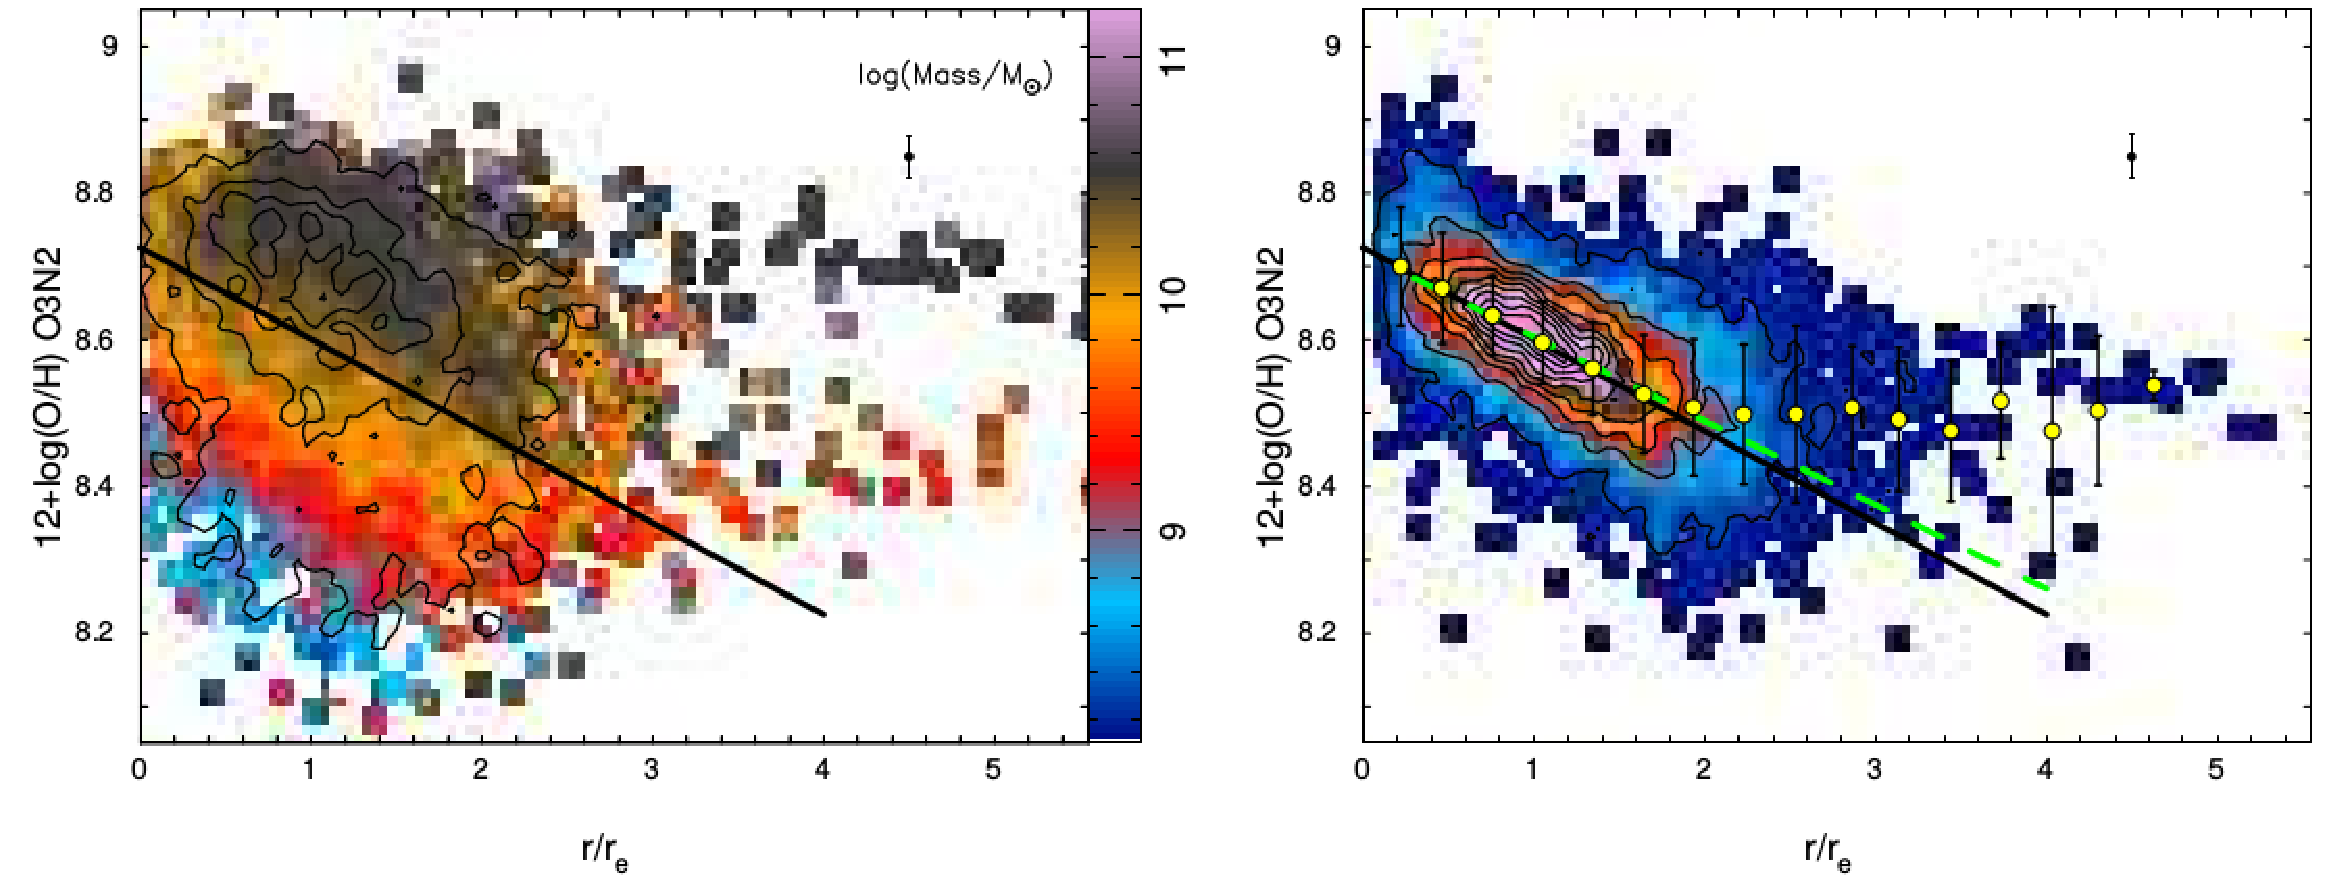
\includegraphics[scale=0.45]{figures/sanchez12_fig9.pdf}

    \caption{Figure 9 from \citet{sanchez12}.\/}

\end{figure*}
\begin{multicols}{2}
%-----------------------------Figure End------------------------------

%-------------------------------------------------------------------------------
\section{The Experiment}
%-------------------------------------------------------------------------------


    \citet{sanchez12} The results of this paper show that disk galaxies in the
    local Universe present a common or character- istic gradient in the oxygen
    abundance of $\alpha$ O/H = -0.1 dex/r e up to $\sim$2 disk effective radii,
    with a small dispersion compatible with being produced by random
    fluctuations


%-------------------------------------------------------------------------------
\subsection{Finding \hii\ Regions and Determining Metallicity}
%-------------------------------------------------------------------------------

    Before drawing conclusions, we will spatially bin the more resolved
    galaxies in our sample so that we can compare the effects of resolution.

    Determining the presence and locations of \hii\ regions in a sample of
    10,000 galaxies is a daunting task. We will adopt the methods of
    \citet{sanchez12} using the code \textsc{HIIexplorer}. The most common
    diagnostic diagram in the literature for the optical regime is the one
    which makes use of easily- observable strong lines that are less affected
    by dust attenuation, i.e., [O\iii]/\,H$\beta$ vs. [N\ii]/H$\alpha$
    (Baldwin et al. 1981)

%-------------------------------------------------------------------------------
\subsection{Deriving Dark Matter Profiles}
%-------------------------------------------------------------------------------



%-------------------------------------------------------------------------------
\subsection{Expected Results}
%-------------------------------------------------------------------------------

%-------------------------------------------------------------------------------
\section{Technical Justification}
%-------------------------------------------------------------------------------

\begin{comment}

%-----------------------------Table Start-----------------------------
\begin{table}[!ht]
\begin{center}
\caption[]{\em{Here we show the continuum sensitivity required per band.}\/}
\begin{tabular}{cc}
\hline \noalign{\smallskip}
Frequency (GHz) & Sensitivity (mJy) \\
\hline \noalign{\smallskip}
100 & 0.01 \\
300 & 0.10 \\
%\hline \noalign {\smallskip}
\end{tabular}
\end{center}
\end{table}
%-----------------------------Table End ------------------------------

You can structure the scientific justification using the two subsections below (optional).

\subsection{Scientific rationale:}

% Please describe the scientific background of the project,
% pertinent references and previous work relevant to this 
% proposal.

\subsection{Immediate objective:}

% Please describe the observations to be made and their specific
% purpose, with a clear explanation of the need for, and 
% appropriateness of, ALMA Cycle 1 data.  

%%%%%%%%%%%%%%%%%%%%%%%%%%%%%
%% Potential for Publicity %%
%%%%%%%%%%%%%%%%%%%%%%%%%%%%%

\section{Potential for Publicity}

% Here, include a brief statement on the potential of your proposal
% to generate publicity based on the scientific results to be obtained.


%%%%%%%%%%%%%%%%%%%%%%%%
%% References section: %
%%%%%%%%%%%%%%%%%%%%%%%%

\section{References}

% List references here

Sanchez cited here \citet{sanchez12}

    \end{comment}

    \bibliography{my_bib}
    
\end{multicols}

%%%%%%%%%%%%%%%%%%%%%%%%%%%
%%%%% End of document %%%%%
%%%%%%%%%%%%%%%%%%%%%%%%%%%

\end{document}

